\documentclass[livre]{udes-genie-these}

\usepackage[T1]{fontenc}
\usepackage{booktabs}
\usepackage{url}  % Enables the use of \url{}
\usepackage{graphicx}
\usepackage{color,soul}
\usepackage{lscape} % For landscape orientation

\ConfigurationDocument
{
  langue = francais,
  type = dprmaitrise,
  programme = electrique,
  lignes,
  liste-figures,
  % liste-tableaux,
  fichier-resume-francais = {resume-francais},
  %fichier-resume-anglais = {resume-anglais},
  % fichier-remerciements = {merci},
  % fichier-lexique = {lexique},
  % fichier-symboles = {symboles},
  fichier-acronymes = {acronymes},
  fichiers-references = {references},
  auto-bib,
  style-references = plain,
}

\TitreFrancais{DÉTECTION DES MOMENTS SAILLANTS D'UNE VIDÉO EN UTILISANT UNE REPRÉSENTATION TEXTUELLE}
\Auteur{Alexandre}{LAFLEUR}
\Date{Avril}{2025}
\MotsClesFrancais{Intelligence artificielle, résumé vidéo, LLM}

\Directeur{François}{GRONDIN}
\Evaluateur{François}{MICHAUD}
\Evaluateur{François}{FERLAND}

\begin{document}

\chapter{INTRODUCTION}

Le développement grandissant de systèmes robotiques autonomes, comme les drones, les bases mobiles et les véhicules autonomes, demande des capacités d'analyse vidéo de plus en plus performantes. Les flux vidéo continus captés par ces plateformes représentent une source considérable de données, dont l'exploitation,  en temps réel ou même en différé, constitue un défi majeur. Principalement dû à des contraintes inhérentes aux systèmes embarqués, comme leur puissance de calcul limitée, leur autonomie énergétique restreinte et leur capacité de stockage souvent réduite. En conséquence, les méthodes traditionnelles d'analyse multimodale, qui combinent à la fois le traitement d'images et le traitement de l’audio, demeurent difficilement applicables sur des dispositifs robotisés contraints en ressources.

L'identification de segments pertinents dans une longue séquence vidéo peut être vu comme un aspect important de la robotique mobile. La détection de moments forts ou événements importants s'avère particulièrement utile dans des sitations de navigation autonome, dans la reconnaissance de situations critiques, dans l’inspection automatisée d'infrastructures ou encore dans la surveillance en milieu complexe et changeant. Pour réaliser cette tâche efficacement sur un robot doté d'un ordinateur embarqué, l'approche conventionnelle, qui repose sur l'analyse directe des flux d'images et de sons à l'aide de modèles spécialisés en vision par ordinateur et en analyse audio, peut présenter plusieurs limites. La lourdeur computationnelle associée, la complexité d'intégration des modèles multimodaux dont la sortie est difficile à contraindre avec précision ou un comportement déterminé à cause de leur plus grande complexité interne, et la difficulté de maintenir un traitement temps réel sur des plateformes matérielles à faible capacité sont tous des bonnes raisons pour essayer de trouver une alternative.

Dans ce contexte, une alternative émergente consiste à exploiter les avancées récentes obtenues avec les grands modèles de langage (LLM), qui atteignent maintenant un niveau remarquable en matière de compréhension et d'analyse sémantique de textes. Pour ce faire, cette recherche propose de convertir l'intégralité des données audiovisuelles issues d'un robot en une représentation purement textuelle pour que le traitement analytique soit confié exclusivement à un modèle linguistique, réduisant ainsi la dépendance aux méthodes multimodales complexes et coûteuses en ressources. 

Cependant, cette solution soulève quand-même plusieurs questions techniques et scientifiques importantes. Premièrement, il est très important que la représentation textuelle de la vidéo reste fidèle et exhaustive, pour permettre une analyse complète de la situation. Une description textuelle complète nécessite non seulement de retranscrire fidèlement les dialogues ou les voix hors champ, mais également de capter efficacement les informations visuelles et non verbales telles que les expressions faciales, le langage corporel, les éléments contextuels et les transitions scénaristiques. Deuxièmement, il reste à déterminer si un modèle de langage peut, à partir de ces représentations textuelles, identifier correctement et automatiquement les moments clés d'une vidéo, avec une précision comparable à celle obtenue par un humain.

L'objectif scientifique principal est de démontrer la faisabilité technique d'un processus entièrement textuel de détection d'événements, adapté aux contraintes spécifiques des plateformes robotiques. En cas de succès, une telle méthodologie permettrait aux systèmes robotiques disposant de ressources limitées de mieux gérer l'identification des événements importants dans des flux vidéo continus, tout en préservant une précision satisfaisante. À plus long terme, cette approche pourrait être utilisée pour ajouter des nouvelles fonctionnalités à des produits dans d’autres domaines qui nécessitent une analyse vidéo efficace à faible coût computationnel.

Pour valider cette approche, l’équipe de recherche créerait et utiliserait une base de données de vidéos existantes, et les associeraient avec leurs segments courts populaires respectifs. Le choix de cette base de données serait lié à la quantité importante de données disponibles et l’adéquation de ces données pour atteindre l'objectif visé. Une validation rigoureuse des résultats obtenus permetterait d’évaluer objectivement la performance du modèle de langage choisi et de la représentation textuelle des vidéos, afin d’itérer facilement et de prouver leur efficacité avant une éventuelle intégration en contexte robotique réel.

Le chapitre 2 présente l’étât de l’art de la situation, le chapitre 3 analyse les solutions existantes, le chapitre 4 explique la problématique en détails, le chapitre 5 propose une approche pour régler la problématique et le chapitre 6 montre une méthodologie et un échéancier possible pour mener à terme la maitrise.


\chapter{Synthèse des contributions pour l’extraction automatique de moments clés dans les vidéos longues}


L'analyse des moments saillants dans les flux vidéo robotiques par approche textuelle répond aux contraintes spécifiques des systèmes embarqués. Les travaux présentés dans cet état de l'art ont été sélectionnés pour leur pertinence dans l'adaptation des méthodes d'analyse vidéo aux ressources limitées des plateformes robotiques. La conversion des données audiovisuelles en représentations textuelles pour traitement par des modèles de langage offre une alternative aux approches multimodales traditionnelles. Les fondements techniques exposés dans les sections suivantes établissent le cadre nécessaire au développement d'une solution d'analyse vidéo textuelle performante dans un contexte de robotique embarquée.

\section{Modélisation vidéo-textuelle et multimodale pour la sélection de clips}

Pour réussir à trouver les moments saillants d’une vidéo, une IA pourrait devoir analyser et comprendre le contenu vidéo, non seulement en termes de ce qui est vu à l’écran, mais également en intégrant les éléments textuels et auditifs de la vidéo. Cette section explore les modèles et techniques vidéo-textuelles et multimodales qui permettent d’enrichir la pertinence et la précision de la sélection des segments dans le cadre de l’automatisation du montage. 

Des modèles comme CLIP \cite{bain2022}(\textit{Contrastive Language Image Pre-training}) et BuboGPT \cite{anonymous2023_bubogpt} jouent un rôle fondamental dans la correspondance entre le contenu visuel et les descriptions textuelles. CLIP a été développé pour relier directement des images à des textes, permettant une correspondance directe entre des concepts visuels et des descriptions narratives. Cette capacité est précieuse pour un résumé automatique, car elle permettrait de sélectionner les segments visuels les plus pertinents par rapport aux requêtes textuelles ou aux tendances narratives \cite{chen2023}\cite{ghosh2019_excl}. Cependant, CLIP est principalement entraîné sur des images statiques, ce qui limite sa capacité à traiter efficacement les dimensions temporelles et narratives des vidéos.


Dans un montage vidéo, la continuité visuelle et le contexte narratif sont essentiels, et cette lacune peut réduire la pertinence des segments identifiés. BuboGPT, quant à lui, renforce cette capacité en ajoutant une couche d’ancrage visuel, permettant une identification et une localisation précises des objets dans chaque image en fonction des descriptions textuelles \cite{feng2023}\cite{munasinghe2023_pgvideo}. Par exemple, une scène de nature pourrait être identifiée et extraite si elle est associée à un texte comme « aventure en plein air ». Cette granularité fine est un atout, mais elle dépend fortement de la qualité des descriptions textuelles fournies. Si les textes sont vagues, ambigus ou contradictoires, le modèle risque de sélectionner des segments non pertinents, réduisant ainsi l’efficacité du montage. 

Si l’image et le texte offrent des informations importantes pour la sélection des segments, l’intégration de l’audio permet une compréhension encore plus riche de la vidéo \cite{anonymous2023_videollama}\cite{han2024_clip}. Les modèles Valley \cite{anonymous2023_valley} et Video-LLaMA \cite{anonymous2023_videollama} démontrent comment des signaux auditifs peuvent être exploités en parallèle des indices visuels et textuels pour un alignement complet des modalités. Valley utilise un alignement multimodal qui intègre des signaux audio pour fournir une compréhension contextuelle approfondie des vidéos \cite{huang2024_vtimellm}, tandis que Video-LLaMA emploie des modules spécialisés qui séparent et intègrent les indices visuels et auditifs en requêtes interprétables par les modèles de langage \cite{xu2024}. Cette approche permet de prendre en compte des éléments sonores tels que les dialogues, les changements d’intonation et la musique, qui influencent fortement l’engagement émotionnel et narratif. 

Cependant, l’efficacité de ces modèles dépend de la qualité des signaux audio disponibles. Par exemple, dans des environnements bruités ou des vidéos amateurs, la performance de Valley peut diminuer, compromettant ainsi la précision de l’analyse contextuelle. De plus, Video-LLaMA, bien que très performant, est coûteux en termes de calcul, ce qui peut le rendre moins adapté à des vidéos longues ou à des systèmes nécessitant des réponses en temps réel. La fusion multimodale de ces approches (image-texte-audio) ouvre la voie à une sélection de clips qui ne se limite pas aux caractéristiques visuelles d’une vidéo, mais qui intègre une compréhension complète des signaux auditifs et textuels \cite{wang2024_hawkeye}\cite{anonymous2017_localizing}. 

Néanmoins, l’intégration de multiples modalités peut également introduire des biais ou des conflits entre les signaux. Par exemple, une musique dramatique superposée à des visuels calmes pourrait créer une ambiguïté dans l’interprétation de la scène. La capacité des modèles à hiérarchiser ces signaux ou à arbitrer entre eux reste un défi à relever.

\section{Localisation et segmentation temporelle des moments clés}

Pour garantir une continuité narrative et un résumé fluide, il faut être capable d’identifier non seulement les moments clés dans une vidéo, mais également leurs limites temporelles précises. Les techniques de localisation temporelle et de segmentation des vidéos jouent ici un rôle essentiel, permettant à l’IA de découper les séquences tout en conservant leur sens et en respectant la chronologie narrative. Cette section explore les approches avancées de segmentation temporelle et de localisation des moments clés, nécessaires pour une sélection précise et cohérente. 

Les modèles comme VTimeLLM \cite{huang2024_vtimellm} et VTG-LLM (\textit{Video Temporal Grounding}) \cite{guo2024_vtgllm} apportent des solutions novatrices pour la délimitation précise des segments vidéo en intégrant des indicateurs temporels explicites. VTimeLLM, par exemple, utilise une stratégie d’entraînement en plusieurs étapes pour renforcer la précision temporelle, permettant de mieux comprendre les débuts et fins des segments d’intérêt \cite{han2024_clip}\cite{lei2021_clipbert}. VTG-LLM, quant à lui, exploite des incorporations (\textit{embeddings}) de séquence-temps et des jetons de temps absolus pour ancrer précisément les moments dans le temps, évitant ainsi les erreurs de quantification qui peuvent survenir dans des vidéos complexes ou de longue durée \cite{guo2024_vtgllm}\cite{you2023_ferret}. 

Cette intégration de l’horodatage permet au modèle de maintenir une continuité temporelle, essentielle pour les montages vidéo nécessitant une précision d’alignement entre les scènes. Ces modèles démontrent l’importance de la localisation temporelle dans les vidéos longues. En intégrant l’horodatage de manière explicite, il serait alors possible non seulement de sélectionner les moments clés avec une plus grande précision, mais aussi de s’assurer que chaque segment est correctement positionné dans l’ordre narratif, évitant ainsi les coupures abruptes ou incohérentes \cite{lei2021_clipbert}\cite{anonymous2017_localizing}. 

Pour organiser les segments dans un ordre fluide, des modèles comme le Moment Context Network (MCN) \cite{anonymous2017_localizing} et 2D-TAN (\textit{Temporal Adjacent Networks}) \cite{zhang2020_temporal} utilisent des techniques de cartographie temporelle et contextuelle. MCN associe des caractéristiques locales et globales pour identifier des débuts et fins de moments spécifiques, en analysant non seulement chaque segment individuellement, mais aussi en tenant compte du contexte général de la vidéo \cite{zhang2016_lstm}\cite{zhang2019_memory}. 2D-TAN adopte une approche de cartographie bidimensionnelle pour modéliser les relations temporelles entre segments adjacents, garantissant ainsi que chaque segment sélectionné conserve une continuité narrative par rapport aux autres \cite{prabhu2017_retrieval}\cite{zhang2020_temporal}.

\section{Détection des faits saillants et filtrage du bruit}

Pour être capable de repérer les moments saillants et de filtrer les segments de moindre intérêt ou redondants, plusieurs modèles ont été explorés. Ils se concentrent sur la détection des faits saillants et l’élimination des segments non pertinents, permettant ainsi une sélection précise des passages qui ont le plus de chances d’être intéressants. 

HL-CLIP \cite{han2024_clip} et GPTSee \cite{sun2023_gptsee} sont deux modèles innovants pour la détection des faits saillants. HL-CLIP utilise une technique de regroupement par saillance (\textit{saliency pooling}) pour stabiliser la détection de moments intéressants en moyennant les scores de saillance à travers plusieurs trames adjacentes. Cette approche permet une détection plus robuste des segments pertinents, même dans des séquences complexes, et évite les sélections incohérentes \cite{you2023_ferret}\cite{sun2023_gptsee}. GPTSee, quant à lui, repose sur une analyse de similarité sémantique entre les descriptions des images extraites et les requêtes textuelles pour identifier les moments saillants les plus engageants \cite{sun2023_gptsee}\cite{liu2022_umt}. 

En ajoutant un filtrage sémantique, GPTSee affine la sélection pour ne retenir que les segments en lien direct avec les thèmes ou intentions de la narration. HL-CLIP et GPTSee démontrent comment la détection de faits saillants peut être renforcée par des scores de similarité et de saillance, améliorant ainsi la pertinence des extraits retenus pour le montage. 

Dans le domaine du filtrage de contenu, LLoVi (\textit{Language-based Long-range Video question answering framework}) \cite{zhang2023} propose une méthode de résumé multi-étapes pour éliminer le bruit et affiner la qualité des segments choisis \cite{anonymous2023_valley}\cite{zhang2019_memory}. L’approche de LLoVi consiste à générer des descriptions textuelles pour chaque clip court, puis à les résumer en plusieurs étapes pour éliminer les informations redondantes ou non pertinentes. Ce processus de résumé successif permet de concentrer l’attention sur les passages ayant la plus forte valeur narrative. 

\section{Fusion multimodale et alignement pour une narration cohérente}

Pour maximiser les chances qu’un passage vidéo soit réellement l’un de ses moments forts, il pourrait être utile d’intégrer des informations provenant de plusieurs modalités en une seule structure cohérente, qu’elles soient visuelles, textuelles ou auditives. La fusion multimodale et l’alignement des informations semblent donc essentiels pour sélectionner des clips à fort potentiel d’être intéressants. Dans cette section, nous explorons les techniques qui permettent d’enrichir la narration vidéo en utilisant des approches multimodales sophistiquées. 

Les modèles UMT (\textit{Unified Multi-modal Transformers}) \cite{liu2022_umt} et Slot-VLM \cite{xu2024} offrent des solutions complètes pour intégrer des informations visuelles, textuelles et auditives dans une seule structure cohérente. UMT exploite les données audio et visuelles pour extraire des moments spécifiques en fonction des requêtes textuelles, en intégrant un générateur et un décodeur de requêtes pour transformer les attentes narratives en points de détection temporels \cite{liu2022_umt}. Cette méthode de fusion permet de traiter les vidéos comme un ensemble multimodal complet, assurant que les segments sélectionnés tiennent compte de tous les signaux disponibles.

Slot-VLM  \cite{xu2024} introduit une autre dimension avec son système de \textit{SlowFast Slots}, qui décompose les vidéos en jetons centrés sur les objets (\textit{slow-slots}) et jetons centrés sur les événements (\textit{fast-slots}). Cette technique permet d’adapter l’analyse des vidéos selon la fréquence d’apparition des objets et la dynamique temporelle des événements, en maintenant une cohérence entre les objets fixes et les mouvements rapides. Cette approche est particulièrement utile pour une narration fluide, car elle prend en compte les éléments stables, comme les décors, et les éléments en mouvement, assurant une transition naturelle entre les segments.

Les modèles ExCL (\textit{Extractive Clip Localization}) \cite{ghosh2019_excl} et QD-DETR (\textit{Query-Dependent DEtection TRansformer}) \cite{sun2023_gptsee} permettent d’adapter dynamiquement les choix de segments en fonction des descriptions narratives et des requêtes textuelles. ExCL utilise une approche extractive qui prédit les trames de début et de fin en fonction de la pertinence avec les descriptions narratives. Ceci permet de sélectionner des segments qui s’alignent étroitement avec les attentes narratives, assurant que chaque clip choisi apporte une valeur ajoutée à la continuité de l’histoire. 

QD-DETR utilise un encodeur à attention croisée qui intègre explicitement les requêtes dans la représentation des clips vidéo, offrant un niveau d’adaptabilité élevé pour correspondre précisément aux intentions narratives des spectateurs \cite{lei2021_moments}. Grâce à un mécanisme d’appariement flexible, il est possible de discriminer entre les segments en fonction de la demande, filtrant les moments qui ne correspondent pas aux critères recherchés.

\section{Optimisation des modèles et traitement des vidéos longues}

Pour les vidéos de longue durée, il serait essentiel d’optimiser les ressources sans compromettre la précision de la sélection des segments. Il faudrait non seulement pouvoir identifier les moments clés dans des vidéos longues, mais aussi le faire de manière efficace et rapide. Les modèles suivants se concentrent sur des techniques d’optimisation qui permettent un traitement plus rapide et moins gourmand en ressources, tout en maintenant une sélection de clips pertinente. 

Les modèles LongVLM \cite{weng2024} et \textit{Less is More}(CLIPBERT) \cite{lei2021_clipbert} mettent en avant des techniques d’échantillonnage éparse et de segmentation optimisée pour éviter le traitement de chaque trame dans les vidéos longues. LongVLM segmente les vidéos longues en clips courts et extrait pour chaque segment les caractéristiques locales, avant de les fusionner dans un contexte global \cite{weng2024}. Cette approche réduit le volume de données à traiter tout en maintenant une compréhension précise des segments. 

\textit{Less is More}(CLIPBERT), quant à lui, utilise un échantillonnage éparse pendant l’entraînement pour capturer les informations essentielles tout en réduisant les besoins en mémoire. Lors de l’inférence, CLIPBERT applique un échantillonnage dense, permettant ainsi de conserver un haut niveau de précision dans la sélection des moments saillants sans traiter chaque trame individuellement \cite{lei2021_clipbert}. En utilisant des méthodes d’échantillonnage et de segmentation, il serait possible de traiter les vidéos longues de manière efficace, en s’assurant que seuls les segments pertinents sont extraits. Par exemple, dans un enregistrement de caméra de surveillance ou dans un flux vidéo de la caméra embarquée d’un robot de plusieurs heures, cette optimisation permettrait de cibler des moments clés sans engorger les ressources de traitement.

Les modèles VTG-LLM \cite{guo2024_vtgllm} et VTimeLLM \cite{huang2024_vtimellm} utilisent des techniques de compression des données visuelles pour réduire la surcharge de traitement sans sacrifier la qualité de l’information. VTG-LLM introduit une compression par compartiment  (\textit{slot}) qui regroupe les informations visuelles en blocs, permettant un échantillonnage étendu avec une capacité de traitement plus élevée \cite{guo2024_vtgllm}. Cette technique est particulièrement utile pour les vidéos longues et complexes, où chaque bloc compressé conserve des détails essentiels pour la narration. 

VTimeLLM, de son côté, utilise une stratégie d’entraînement par étapes pour améliorer la localisation temporelle dans des vidéos longues, permettant ainsi de mieux appréhender les séquences d’événements sans pertes de données importantes \cite{huang2024_vtimellm}. Grâce à des jetons compressés, ce modèle permet de traiter des vidéos volumineuses tout en conservant une précision optimale. En utilisant des techniques de compression et de traitement par \textit{slots}, il serait possible de gérer de grandes quantités de données sans ralentir le processus de sélection, tout en assurant la précision nécessaire pour maintenir l’intérêt narratif et visuel des clips.

Les techniques d’optimisation proposées par LongVLM \cite{weng2024}, \textit{Less is More}(CLIPBERT) \cite{lei2021_clipbert}, VTG-LLM \cite{guo2024_vtgllm}, et VTimeLLM \cite{huang2024_vtimellm} permettent de réduire considérablement la complexité de traitement dans des vidéos longues, tout en maintenant la qualité de sélection des segments pertinents. 

\section{Intégration et implications pour le développement de la solution}

L’ensemble des techniques et modèles analysés dans cet état de l’art met en lumière les différentes approches et technologies qui peuvent être intégrées pour développer une solution performante, capable de répondre aux attentes actuelles de l’analyse de longues vidéos et de la reconnaissance des moments saillants. Des techniques de modélisation multimodale, de localisation temporelle, de détection de saillance, de fusion des modalités et d’optimisation pour les vidéos longues se complètent pour offrir une solution cohérente et efficace pour régler le problème. En combinant ces approches, il serait possible de : 

1) Analyser des signaux visuels, textuels et auditifs pour sélectionner des segments qui répondent aux attentes narratives et émotionnelles d’un moment qui serait qualifié de saillant \cite{chen2023}\cite{munasinghe2023_pgvideo}. 

2) Maintenir une cohérence narrative en appliquant des techniques de localisation et de segmentation qui assurent des transitions fluides entre les moments sélectionnés \cite{wang2024_hawkeye}\cite{guo2024_vtgllm}. 

3) Optimiser la pertinence des extraits retenus grâce à la détection des faits saillants et au filtrage des segments non pertinents, garantissant un résumé qui capte l’attention tout en restant précis et concis \cite{you2023_ferret}\cite{han2024_clip}. 

4) Traiter efficacement les vidéos longues en appliquant des techniques d’échantillonnage et de compression qui permettent un traitement rapide et moins coûteux en ressources \cite{weng2024}\cite{lei2021_clipbert}.

\chapter{Analyse comparative approfondie et différenciation par rapport aux solutions existantes}

\section{Introduction et contexte}

Sur le web, plusieurs plateformes alimentées par l’intelligence artificielle ont émergé pour simplifier et accélérer le processus de création de clips courts. Ces plateformes offrent aux créateurs de contenu, aux équipes marketing et aux utilisateurs sans compétences techniques avancées la possibilité de générer des clips attractifs, lire ici des moments saillants, à partir de vidéos longues. Même si elles ne sont pas adaptées pour la recherche robotique, elles comblent un besoin très semblable à ceux des chercheurs qui désirent extraire les moments forts du flux vidéo d’un robot. Elles doivent générer un très grand nombre de clips pour un très faible coût monétaire dû à la forte compétition entre plateformes. Ces solutions purement logicielles et automatisées gardent leurs coûts bas en utilisant des modèles de langage optimisés et des techniques de traitement vidéo à faible puissance de calcul. Ce choix technologique est lié aux contraintes rencontrées par les chercheurs en robotique, qui désirent analyser le flux vidéo issu des capteurs embarqués sur des robots disposant de ressources computationnelles limitées. De manière similaire aux plateformes web devant minimiser leurs coûts de calcul, les robots pourraient bénéficier d'approches légères pour assurer une autonomie suffisante tout en conservant des performances acceptables. Ainsi, étudier les techniques employées par ces plateformes web offre des pistes utiles pour développer des méthodes d'analyse vidéo adaptées aux systèmes embarqués aux ressources limitées.

Parmi les solutions principales, Descript \cite{descript2024}, Captions.ai \cite{captions2024}, 2short.ai \cite{short2024}, Ssemble \cite{ssemble2024}, OpusClip \cite{opusclip2024}, Powder \cite{powder2024}, Munch \cite{munch2024}, Klap \cite{klap2024}, Framedrop \cite{framedrop2024}, SendShort \cite{sendshort2024}, et Recast Studio \cite{recast2024} se distinguent par leurs approches variées dans le domaine de l’automatisation de l’édition vidéo. Chaque plateforme propose des fonctionnalités spécifiques pour répondre aux besoins d’engagement, de viralité et d’accessibilité, capitalisant sur des technologies IA telles que la transcription, la segmentation vidéo, l’édition basée sur des critères de popularité et la personnalisation partielle des clips.

\section{Approches et technologies utilisées par les solutions existantes}

Les plateformes d’édition vidéo automatisée reposent sur une série de technologies et d’approches IA variées pour analyser, sélectionner et transformer des vidéos longues en clips courts adaptés aux réseaux sociaux. Descript \cite{descript2024} se distingue dans le domaine de l’édition vidéo en proposant une interface qui permet de modifier directement le contenu vidéo à partir de la transcription texte, une innovation qui rend l’édition de contenu aussi intuitive que la modification d’un document texte. En intégrant une transcription rapide et précise des fichiers audio et vidéo, Descript simplifie la création de contenu en offrant une base textuelle pour éditer et réviser les enregistrements. La simplicité d’utilisation et la rapidité de la transcription permettent aux utilisateurs d’éditer les vidéos de manière efficace, sans avoir à manipuler directement les clips vidéo. Cette approche basée sur le texte, bien que puissante, enlève tout l’aspect visuel de la vidéo et requiert souvent une deuxième édition visuelle pour les détails plus fins.

Captions.ai \cite{captions2024}, 2short.ai \cite{short2024}, Ssemble \cite{ssemble2024} et OpusClip \cite{opusclip2024} automatisent l’extraction des moments clés d’une vidéo, en analysant des indicateurs d’engagement et de viralité pour sélectionner les segments qui ont le plus de potentiel de capter l’attention d’une personne qui regarde la vidéo. Ces outils scannent le contenu vidéo et identifient automatiquement les moments saillants en fonction de critères préétablis, offrant aux créateurs un moyen rapide de créer des clips engageants. Ces technologies permettent un gain de temps considérable pour les créateurs de contenu, réduisant la nécessité d’explorer manuellement la vidéo pour trouver les moments engageants.

2short.ai \cite{short2024}, Framedrop \cite{framedrop2024}, Powder \cite{powder2024} et Munch \cite{munch2024} se concentrent sur des techniques de détection et de retouche visuelle, comme le suivi facial ou l’ajout d’effets visuels et sonores. Par exemple, 2short.ai utilise la technologie de suivi facial pour garder le focus sur les intervenants principaux, ce qui améliore l’impact visuel, tandis que Powder \cite{powder2024} se concentre sur les enregistrements de jeux vidéo en détectant les moments d’action et en appliquant des modèles de montage spécifiques au contenu de jeu. Ces outils permettent d’améliorer l’impact visuel en utilisant des ajustements centrés sur les éléments clés, comme les visages ou les objets importants, tout en optimisant la vidéo pour des plateformes spécifiques. Par contre, ces fonctionnalités peuvent être restreintes à des types de contenu particuliers, ce qui limite leur utilisation pour des vidéos plus variées.

Klap \cite{klap2024}, SendShort \cite{sendshort2024} et Recast Studio \cite{recast2024} permettent aux utilisateurs de personnaliser les clips en ajoutant des effets visuels et des légendes afin de renforcer l’identité visuelle du contenu. Bien que chaque plateforme offre des options de personnalisation, elles sont souvent limitées à des ajustements de base et peuvent nécessiter des compétences en édition pour des modifications avancées. Cette personnalisation permet aux utilisateurs de mettre encore plus en valeur une partie de la vidéo, comme pour un robot qui voudrait mettre un carré rouge autour de la chose précise qu’il a remarquée qu’était anormale.

\section{Avantages et limites des solutions existantes}

Les plateformes d’édition vidéo automatisée telles que Descript \cite{descript2024}, Captions.ai \cite{captions2024}, 2short.ai \cite{short2024}, Ssemble \cite{ssemble2024}, OpusClip \cite{opusclip2024}, Powder \cite{powder2024}, Munch \cite{munch2024}, Klap \cite{klap2024}, Framedrop \cite{framedrop2024}, SendShort \cite{sendshort2024}, et Recast Studio \cite{recast2024} présentent des avantages notables qui les rendent intéressants pour des utilisateurs voulant générer rapidement des clips à partir de longs vidéos. La majorité des plateformes existantes offrent une interface intuitive, simplifiant l’édition vidéo même pour les utilisateurs novices. L’automatisation des tâches de segmentation, d’extraction de moments clés et d’ajout de sous-titres réduit le besoin de compétences avancées en montage vidéo. Ceci rend ces plateformes idéales pour ceux qui souhaitent produire rapidement des clips sans maîtriser les outils d’édition traditionnels.

Les outils d’ajustement et d’optimisation sont spécifiquement conçus pour maximiser l’attention, en créant des clips dynamiques qui captent l’attention de l’audience. Un robot qui génère un clip de ce genre aurait plus de chance que son clip soit écouté au complet, ce qui maximiserait le transfert d’information humain-machine. Avec la mondialisation du contenu numérique, plusieurs plateformes, comme Captions.ai \cite{captions2024}, OpusClip \cite{opusclip2024} et Framedrop \cite{framedrop2024}, ont intégré le support de plusieurs langues. Cette fonctionnalité permet aux utilisateurs de s’adresser à des audiences diversifiées et d’augmenter leur portée. Les plateformes sont capables de générer des sous-titres dans plusieurs langues et d’inclure des options de traduction, rendant le contenu plus accessible et inclusif.


\chapter{PROBLÉMATIQUE}

D’un côté, les méthodes classiques d'analyse automatisée des contenus vidéo reposent souvent sur des architectures multimodales complexes, intégrant à la fois des traitements visuels, audio et textuels. L’utilisation de grands modèles de langage multimodaux pour la tâche d’analyse vidéo demande des ressources computationnelles significatives, ce qui les rend peu accessibles, spécialement dans des contextes contraints par une capacité limitée de calcul ou de stockage comme les systèmes embarqués en robotique. Il serait important de développer une méthode d’analyse vidéo qui utilise moins de ressources pour faciliter son utilisation en contexte de robotique mobile.
Parallèlement, la popularité des vidéos courtes tirées de longues vidéos, parfois appelées \textit{shorts}, porte à croire que les moments forts (ou saillants) d'une longue vidéo peuvent systématiquement être extraits et isolés comme particulièrement importants. Ce fait, d’apparence non relié au domaine de la robotique, est pourtant un aspect très important à ce projet de recherche. Ces clips extraits de longues vidéos se rapprochent beaucoup des moments intéressants du long flux vidéo que peut produire un robot muni de caméras. Si des données vidéos librement disponibles sur internet et libres de droits peuvent être transcrites au format textuel et utilisées pour entraîner et tester un grand modèle de langage pour la détection de moments forts, un des plus gros problèmes à l’entraînement de ces modèles, le nombre de données astronomique requis pour le faire n’est plus un enjeu.
Donc, en combinant le besoin de méthodes moins énergivores pour l’analyse vidéo en robotique, et la disponibilité d’une base de données très similaire aux besoins de la détection de moments forts sur de longs flux vidéos en robotique, la question de recherche suivante émerge :

Dans quelle mesure est-il possible de représenter fidèlement et exhaustivement le contenu d'une vidéo exclusivement par des descripteurs textuels, afin de permettre à un grand modèle de langage (LLM) d'identifier automatiquement les segments les plus saillants ?
Cette question conduit à deux dimensions interdépendantes de la problématique :

\textbf{1) La fidélité et l'exhaustivité de la représentation textuelle du contenu vidéo}

La principale difficulté réside dans l'identification, puis dans l’octroiement des éléments pertinents à inclure dans la représentation : les actions visibles à l'écran, les dialogues entendus, l’ambiance sonore, les variations émotionnelles, les transitions entre les scènes ou tout autre élément contextuel. Aussi, une réflexion, et surtout une rétroaction, doit être menée sur la granularité optimale de cette représentation textuelle afin d'éviter une perte significative d'information tout en gardant une taille restreinte rester traitable par des modèles de langages avec une petite taille de contexte. 


\textbf{2) La capacité du LLM à identifier les moments clés à partir d'une représentation strictement textuelle}

Le modèle doit être en mesure de détecter des segments porteurs d'intérêt particulier (émotion, intensité narrative, action décisive) sans accès direct aux aspects visuels et sonores d'origine. Il faut alors avoir une façon d’entrainer et de valider le modèle pour cette tâche précise.


Ce qui amène à l'objectif général du projet, qui consiste à vérifier la faisabilité et l'efficacité d'une représentation strictement textuelle des vidéos pour l'identification automatisée de segments clés par un LLM , et ses quatre sous-objectifs:

1) Élaborer une représentation textuelle complète et structurée du contenu vidéo

2) Évaluer la possibilité d’identifier les moments forts, à partir de cette représentation textuelle, d'un grand modèle de langage (LLM)

3) Comparer objectivement les extraits sélectionnés par le modèle avec des extraits de référence.

4) Optimiser progressivement la méthode de représentation textuelle et l'utilisation du modèle afin d'améliorer la concordance avec les références



\chapter{APPROCHE PROPOSÉE, MÉTHODOLOGIE ET ÉCHÉANCIER}

La recherche repose sur l'hypothèse qu'il serait possible de générer une description textuelle suffisamment exhaustive d'une vidéo pour permettre à un grand modèle de langage (LLM) purement textuel d'identifier automatiquement les moments saillants d'une vidéo. Dans le but de minimiser les ressources nécessaires pour l'analyse et pour l'utiliser dans des systèmes embarqués ou des situations de ressources limitées.

\section{Élaboration d'une représentation textuelle structurée}

L'objectif consiste à définir et valider une méthode d'encodage textuel capable de représenter de façon fidèle et précise les dimensions visuelles, auditives et narratives d'une vidéo. Le tout, en restant assez concis pour permettre que le traitement soit fait par un LLM le moins énergivore possible et en utilisant le moins de jetons possible. Une des hypothèses sur laquelle repose cette partie est qu'avec une représentation suffisamment détaillée et avec un choix judicieux des composantes détaillées, le problème d'analyse vidéo pourrait être simplifié, permettant à un modèle moins puissant de l'analyser correctement. En bref, il s’agit d’encoder à l’avance les données jugées pertinentes, pour réduire la charge d’inférence du LLM.

La représentation textuelle inclurait une transcription des dialogues et des narrations, une segmentation temporelle de la vidéo en scènes ou en événements distincts et, si possible, l'inventaire des objets présents dans la scène et des informations sur l'intonation ou sur l'émotion perçue. Il serait important que le tout soit structuré de façon claire et constante pour aider un grand modèle de langage à travailler avec.

Pour ce faire, il faudrait réaliser l'évaluation comparative de plusieurs outils existants en reconnaissance automatique de la parole, par exemple Whisper \cite{radford2023_whisper}. et des modèles de reconnaissance visuelle d'objets et de scènes, basés sur des réseaux neuronaux pré entraînés disponibles dans la littérature, par exemple les modèles convolutifs comme YOLOv12 \cite{tian2025yolov12}. Le choix final des outils sera justifié par une analyse quantitative de leur précision (taux d'erreur des transcriptions ou taux de reconnaissance d'objets validés sur jeux de données publics, comme COCO \cite{lin2014_coco} ou ActivityNet \cite{heilbron2015_activitynet}). 

Il faudrait également mettre en place un prototype de séquence de traitement automatisé combinant tous les outils. L'efficacité de cette combinaison sera validée en mesurant le nombre de ressources utilisées, afin de s'assurer que la séquence de traitement complète qui permet d'utiliser un LLM purement textuel n'est pas en fait plus gourmand en ressources qu'un LLM multi-modal. Il faudrait alors comparer l'usage en ressources d'un LLM multi-modal pour une même vidéo, et pour une analyse vidéo avec une précision et exactitude similaire. 

La validation se fera sur un échantillon réduit de vidéos libres de droits choisis par les chercheurs, afin d'ajuster empiriquement la granularité optimale et les éléments présents dans la représentation. On saura que la représentation fonctionne quand le LLM pourra l'utiliser pour extraire un moment de façon constante. Ce sera alors dans la dernière étape d'itération et d'optimisation que la représentation textuelle pourra être testée davantage et modifiée pour obtenir de meilleurs résultats, soit des moments plus saillants, plus proches de ceux choisis dans la base de données.

\section{Utilisation d'un grand modèle de langage pour identifier les segments clés}

Pour cet objectif, il faut faire la sélection d'un LLM approprié et l'évaluation rigoureuse de sa capacité à localiser correctement les segments clés, en comparant ses résultats à une référence établie par les chercheurs. Le but est de vérifier, parmi les modèles de langage existants, lequel peut répondre le plus adéquatement à la tâche d'analyse vidéo via représentation textuelle, et de vérifier de quelle façon il est possible d'augmenter les capacités d'un modèle pré-entraîné pour réaliser la tâche spécifique en utilisant différents principes d'ajustements fins et d'interrogations du modèle.

Le modèle retenu (par exemple GPT-4) traitera chaque description selon une consigne unique et standardisée. La validation se fera quantitativement. Un indice d'intersection temporelle sera utilisé pour quantifier la correspondance entre l'extrait identifié automatiquement par le LLM et l'extrait associé dans la base de données. Cet indice correspond au ratio du chevauchement temporel par rapport à la durée totale de l'extrait de référence. Il est difficile d'estimer adéquatement le seuil acceptable pour cette mesure, mais en utilisant l'hypothèse qu'un moment fort est assez précis dans le temps, mais que le début et la fin d'un moment fort peuvent être un peu floues dépendamment du niveau de contexte voulu, un seuil de 10 pour cent semble adéquat pour la problématique.  Ce choix de mesure se justifie par sa simplicité et sa fréquence d'utilisation en localisation temporelle dans la littérature existante.



\section{Comparaison des résultats avec des références existantes}

Cette section vise à mesurer concrètement si les choix effectués par le modèle concordent avec les moments considérés comme saillants par la base de données, qui elle-même serait créée à partir de vidéos libres de droits disponibles en ligne. Il faudrait d'abord monter cette base de données, puis l'utiliser pour comparer la performance des différentes représentations et modèles. Selon LIMA \cite{zhou2023lima}, la qualité, la diversité et la spécificité de format des données ont plus d’impact que la taille brute du jeu de données sur la performance du modèle. Après milles exemples bien choisis, les bénéfices d’en ajouter d’autres sont négligeables.

Le corpus inclura des vidéos et des extraits courts libres de droits provenant de la plateforme YouTube, sélectionnées selon les critères suivants : Diversité des genres (documentaires, tutoriels, humour, vlogs), afin de tester la robustesse de l'approche face à différents contextes, puisqu'un robot peut être utilisé dans toutes sortes de situations. Présence d'extraits courts (\textit{shorts}) déjà populaires, servant de référence externe fiable pour l'évaluation du modèle. Chaque vidéo retenue ainsi que ses extraits courts associés seront convertis à un format textuel avec des horodatages en utilisant des outils comme Whisper \cite{radford2023_whisper}. Il faudra alors utiliser des algorithmes de type fenêtre glissante pour trouver où exactement dans la vidéo ce moment fort est-il présent. 

\section{Processus itératif d'optimisation}

Pour cet objectif, un processus itératif sera mis en place pour affiner progressivement la description textuelle, l'entraînement fin et les instructions données au LLM. Chaque itération sera motivée par les performances mesurées à l'étape précédente. Des améliorations pourront inclure l'ajout de descripteurs textuels complémentaires comme les expressions faciales, les nuances émotionnelles ou les annotations temporelles supplémentaires. 

Par exemple, si l'absence d'informations émotionnelles ou contextuelles essentielles, marquée par le fait que l'extrait de référence est hautement chargé en émotion, mais que le LLM ne semble pas être capable d'utiliser cette information pour le trouver, il faudrait procéder à une itération. Dans ce cas, la description textuelle serait enrichie en intégrant des descripteurs supplémentaires (annotations émotionnelles, variations d'intonation), dont l'importance est déjà confirmée par la littérature sur l'analyse multimodale. 

Un éventuel ajustement du modèle de langage avec un entraînement fin sur les données récoltées pourrait être également être envisagé si les premiers résultats démontrent une nécessité claire d'améliorer la sensibilité du modèle aux indices spécifiques au contexte vidéo. Pour ce faire, il faudrait générer une représentation temporelle complète des vidéos de référence afin de se générer des données d'entraînement propres à la situation. Chaque itération serait documentée, justifiée scientifiquement et suivie d'une nouvelle validation selon les mêmes critères quantitatifs et qualitatifs mentionnés précédemment.

\section{Échéancier}

Phase 1 (6 mois): Conception de la représentation textuelle et du protocole d'extraction automatique \newline
Phase 2 (6 mois): Constitution d'une base de données de vidéo et clips associés  \newline
Phase 3 (6 mois): Interaction avec le grand modèle de langage et validation comparative \newline
Phase 4 (6 mois): Processus itératif d'optimisation \newline


\begin{figure}[ht]
  \centering
  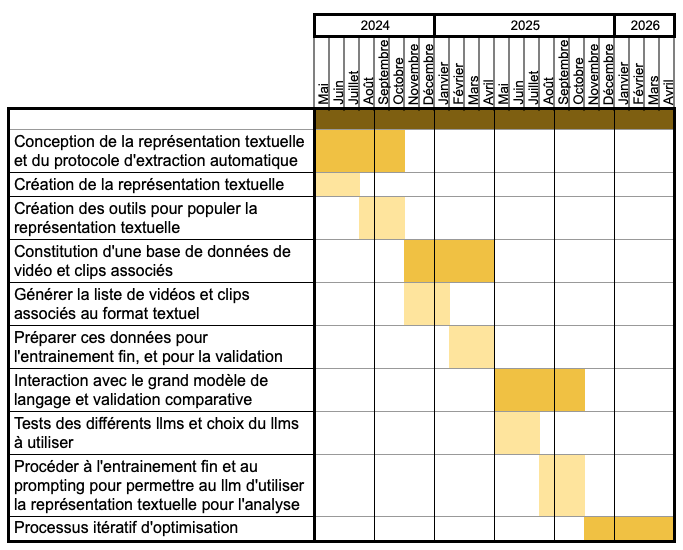
\includegraphics[width=1\textwidth]{gantt.png}
  \caption{Échéancier du projet}
  \label{fig:label}
\end{figure}


\chapter{CONCLUSION}
Cette définition de projet de recherche propose une étude qui vise à déterminer la possibilité de représenter fidèlement et exhaustivement une vidéo par une représentation exclusivement textuelle, pour permettre à un grand modèle de langage (LLM) d'identifier automatiquement les moments les plus pertinents de la vidéo. Le projet vise à utiliser les avancées des grands modèles de langages pour analyser une vidéo en utilisant moins de ressources qu'avec une approche multi-modale plus complexe et coûteuse en ressources. La recherche a pour but d'évaluer si une transcription détaillée, intégrant des éléments visuels, narratifs et sonores sous forme textuelle structurée, permettrait à un LLM de détecter efficacement des événements saillants dans une séquence vidéo. 

Cette question est très importante dans le contexte de la robotique, où les robots sont équipés de systèmes embarqués aux ressources et de caméras. La capacité de ces robots à analyser de longs flux vidéo et à isoler automatiquement des moments clés, sans recourir à des traitements multi-modaux coûteux en ressources donc parfois impossible avec les ressources des systèmes embarqués, représenterait une avancée dans le domaine de la robotique, qui pourrait ouvrir la voie vers des nouvelles fonctionnalités auparavant réservées à l'infonuage. 

Les résultats attendus incluent, entre autres, la validation expérimentale d'une méthodologie permettant de générer des représentations textuelles adaptées à l'analyse automatique par des LLM. Ils incluent également une comparaison rigoureuse entre les extraits identifiés par le modèle et les extraits validés dans la base de données expressément construite pour cette problématique, afin de quantifier la précision et l'efficacité de l'approche. La contribution scientifique majeure de cette étude serait de démontrer que des systèmes purement textuels peuvent effectivement remplacer, dans certaines situations précises, des méthodes multimodales gourmandes en puissance de calcul, tout en conservant une capacité d'analyse satisfaisante. 

Sur le plan pratique, les retombées potentielles incluent la réduction significative des ressources nécessaires pour réaliser l'analyse automatisée de vidéos embarquées sur des plateformes robotiques. De telles avancées ouvriraient la voie à des robots autonomes capables de surveillance intelligente, d'inspection automatisée ou de reconnaissance rapide d'événements critiques dans des environnements variés (sécurité, exploration, assistance aux humains), tout en minimisant les contraintes matérielles et énergétiques. Puisqu'il serait entraîné avec des données provenant de vidéos du quotidien réalisées par des humains, il pourrait s'avérer particulièrement pertinent pour la reconnaissance de situations ou de tensions émotionnelles en présence d'humains, ce qui pourrait contribuer grandement à mieux coexister avec les robots et s'acclimater à leur présence. 

À plus long terme, ce projet contribuerait à la communauté scientifique en clarifiant les avantages et les limites d'une représentation purement textuelle pour des contenus audiovisuels. Il permettrait également de mieux cerner les conditions sous lesquelles l'information visuelle peut être traduite efficacement en descripteurs textuels sans perte critique de données, ainsi que les risques potentiels liés à une simplification excessive.


\end{document}